\pdfoutput=1

\documentclass{l4proj}

%
% put any packages here
%
\usepackage{float}
\usepackage{enumitem}
\usepackage{longtable}
\usepackage{listings}
\usepackage{hyperref}
\usepackage{subfiles}
\usepackage{color}
\usepackage{graphicx}

\newcommand{\nc}[1]{\textcolor{magenta}{(\textbf{NC:} #1)}}
\newcommand{\gac}[1]{\textcolor{cyan}{(\textbf{GAC:} #1)}}
\newcommand{\pwt}[1]{\textcolor{blue}{(\textbf{PWT:} #1)}}

\graphicspath{{images}{../images/}}

\lstdefinestyle{codestyle}{
    %basicstyle=\footnotesize,
    %breakatwhitespace=false,
    breaklines=true,
    %captionpos=b,
    %keepspaces=true,
    %numbers=left,
    %numbersep=5pt,
    %showspaces=false,
    %showstringspaces=false,
    showtabs=false,
    tabsize=2
}

\lstset{style=codestyle}

\begin{document}
\title{Evaluating the Scalability of ROS in Multi-Robot Systems}
\author{Isaac Jordan}
\date{\today}
\maketitle

\begin{abstract}
Robots, distributed systems, and middleware.
\end{abstract}

\educationalconsent
%
%NOTE: if you include the educationalconsent (above) and your project is graded an A then
%      it may be entered in the CS Hall of Fame
%
\tableofcontents
%==============================================================================

\pagebreak
\pagenumbering{arabic}

\subfile{sections/introduction}

%\vspace{-7mm}
%\begin{figure}
%\centering
%\includegraphics[height=9.2cm,width=13.2cm]{uroboros.pdf}
%\vspace{-30mm}
%\caption{An alternative hierarchy of the algorithms.}
%\label{uroborus}
%\end{figure}

\chapter{Background}
\label{background-chapter}

\subfile{sections/background-part1}

\subfile{sections/background-part2-middleware-overview}

\subfile{sections/background-part3-middleware-discussion}

\subfile{sections/background-part4}

\chapter{Communication Scalability}
\label{communication-chapter}

Multi-robot systems are types of distributed systems. The main concern in moving from a single-host distributed system to a multi-host distributed system is the introduction of more complex communication network. As the overall system is trying to complete a task, the individual nodes in the network must communicate in order to share things like the status of the node (CPU load, disk usage, etc), progress through the current task, and results of a task. The exact nature and direction of this communication is dependent on the architecture of the distributed system.

In ROS, the Master node monitors the progress and status of the other nodes, but does not involve itself in the application logic of the system, meaning that it does not process or handle the results of nodes. This is handled in a peer-to-peer (P2P) fashion dictated by the application developer - each node is responsible for choosing what information to request from other nodes, and what information to emit from itself using the Publisher/Subscriber model described in Section \ref{background-ros}. The consequence of this architecture is that overall system performance can be dramatically affected by the communication performance between nodes.

In order to systematically evaluate how ROS' communication scales, one must first aim to understand which aspects of the system that are of greatest importance to performance - both in terms of latency of messages, and total throughput of communication. Section \ref{communication-scoping-experiments} aims to analyse the performance bottlenecks of a simple multi-robot system when sending very controlled and artificial data. Section \ref{communication-real-data} will then aim to validate the results of Section \ref{communication-scoping-experiments} using realistic (previously recorded) data streams, with the goal that these conclusions wil then be directly applicable to real ROS multi-robot systems.

\begin{table}[H]
\centering
\caption{Chapter \ref{communication-chapter} Experiment Overview}
\label{communication-experiment-overview}
\begin{tabular}{|p{0.25\columnwidth}|p{0.4\columnwidth}|p{0.1\columnwidth}|}
\hline
\textbf{Experiment}         & \textbf{Description}                                                                              & \textbf{Section}              \\ \hline
Revising Existing Code      & Building upon prior work to obtain baseline expectations of ROS communication performance         & \ref{exp-1}                 \\ \hline
Effects of Rebooting        & Identifying whether rebooting the host machines affects performance of repeated message streams   & \ref{exp-2}                 \\ \hline
Effects of CPU Clock Speed  & Identifying whether performance of the message streams is limited by processing power             & \ref{experiment3-cpu-speed} \\ \hline
Effects of Wi-Fi Connection & Investigating the effect of performing ROS communication over a Wi-Fi based communication channel & \ref{exp-4}                 \\ \hline
Effects of CPU Clock Speed when using Representative Data & Aiming to validate the results of the CPU Clock Speed scoping experiment on data more typical of a ROS system  & \ref{exp-5} \\ \hline
Effects of Wi-Fi Connection when using Representative Data & Aiming to validate the results of the Wi-Fi Connection scoping experiment using data more typical of a ROS system & \ref{experiment-6} \\ \hline

\end{tabular}
\end{table}

\section{Scoping Experiments}
\label{communication-scoping-experiments}

In order to acquire a detailed understanding of the performance characteristics of ROS' communication channels, a sequence of scoping experiments was designed. The experiments begin very simply - trying to gain baseline expectations of how well ROS will perform, and where problems may occur. Further experiments then investigate individual experimental parameters to identify problem areas for ROS. These experiments were performed using highly controlled data - specifically a single string consisting of `Hello World'. This allows for rapid development and iteration of experiments, while keep the data sent constant. Later experiments (in Section \ref{communication-real-data}) then explore how varying the data sent affects the conclusions of the scoping experiments.

\subfile{sections/experiment1}

\subfile{sections/experiment2}

\subfile{sections/experiment3}

\subfile{sections/experiment4}

\section{Representative Data Experiments}
\label{communication-real-data}

Previous experiments (in Section \ref{communication-scoping-experiments}) were presented as scoping experiments. These were designed to systematically evaluate and gain understanding of which variables were of concern when running tests on ROS' communication performance. However, it was not certain that these prior conclusions would translate well to using ROS in a realistic scenario since throughout the scoping experiments, the same message of `hello world' was used as dummy data. This is a very small message payload of only 11 bytes.

In order to verify the conclusions were correct, samples of realistic data were explored. Two data types were settled on, `sensor data' and `video data'. Sensor data is the type of data likely the come from a physical sensor on the robot. This data is characterised by small message sizes, such as 4KB. Video data is the type of data recorded from a video camera peripheral, such as a webcam. This type of data generally has larger message sizes in range of hundreds of kilobytes, up to several megabytes per message depending on the resolution and bitrate of the camera.

The exact data sets used in the coming experiments were acquired from the MIT Stata Center dataset \cite{mit-stata-center-dataset}. The dataset is described as follows by the producers of the data: ``The MIT Stata Center Data Set is a vast scale data set collected over a multi-year period in a 10 storey academic building. It contains sensor data collected since January 2011. As of September 2012 the data set comprises over 2.3TB, 38 hours and 42 kilometres (the length of a marathon).''\cite{mit-stata-center-dataset} The data is recorded from sensors on the PR2 (a two-armed wheeled robot), which was one of the first robots to ever be designed using ROS as a middleware. The exact values of the data are not important for this evaluation of ROS, it is only the size and frequency of the messages that are important as there is no analysis or computation being executed on the data being transmitted.

This dataset contains both sensor feeds (from a laser sensor), and video feeds (from a Kinect RGB + depth camera). The sensor data was a 20Hz message stream, which was measured to use 85kB/s of bandwidth, giving an individual message size of 4.25kB. The video data used was a 30Hz (30 frames-per-second) RGB (colour) video stream, with a resolution of 640 x 480 pixels. This message stream was measured to use 9.25MB/s of bandwidth, implying a message size of 308KB. These data sets are very large (20 - 50GB) which would require modification to the test system (Raspberry Pi 3’s). Thus these datasets have been filtered down to 60 seconds of recording, resulting in 1791 camera images, and 1194 LaserScan readings. This number of messages was chosen at it would give a good number of messages to average latency over (over 1000 for each data type), but would also easily fit on to the SD-card storage of the Raspberry Pis, which is only 8GB. The total size of the 60 seconds of data was approximately 1GB.

\subfile{sections/experiment5}

\subfile{sections/experiment6}

\chapter{Host Scalability}
\label{host-scalability-chapter}

These scalability experiments look in to how well ROS scales when introduced to more nodes, or more hosts, or both.

\subfile{sections/experiment7}

\subfile{sections/experiment8}

\subfile{sections/experiment9}



\subfile{sections/conclusion}





%%%%%%%%%%%%%%%%
%              %
%  APPENDICES  %
%              %
%%%%%%%%%%%%%%%%
\begin{appendices}

\chapter{Continued Middlewares Overview}
\label{middlewares-overview-appendix}
\subfile{sections/background-part2-middleware-overview-appendix}

\chapter{Experiment 2 Other Graphs}
\label{exp2-appendix-results}

\begin{figure}
\centering
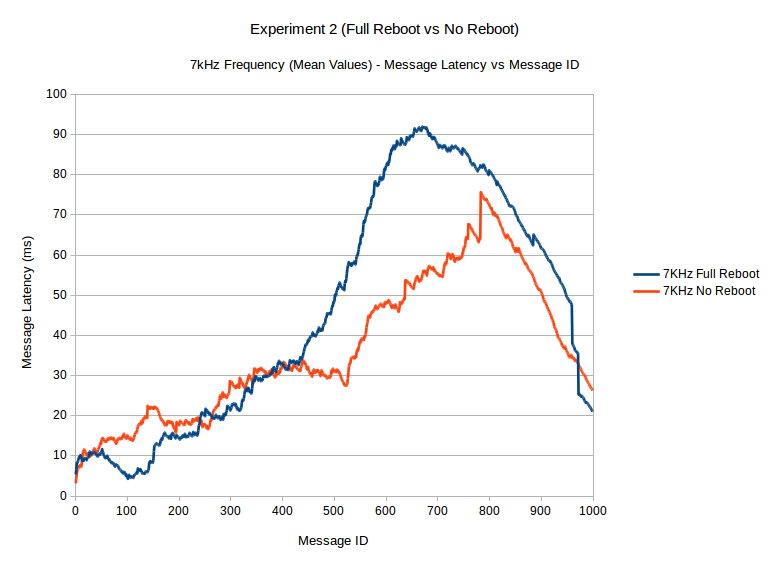
\includegraphics[width=\textwidth]{images/experiment2/7khz-mean.png}
\caption{Experiment 2 - 7KHz Message Frequency}
\label{exp2-7khz}
\end{figure}

\begin{figure}
\centering
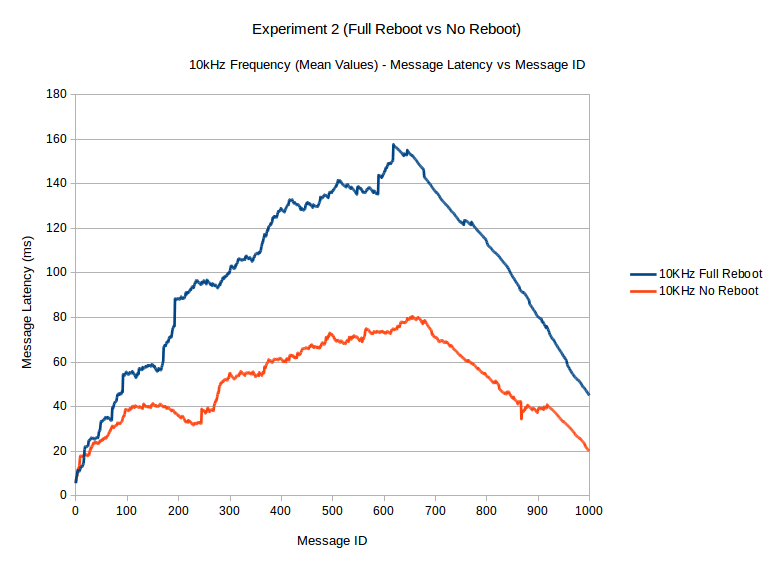
\includegraphics[width=\textwidth]{images/experiment2/10khz-mean.png}
\caption{Experiment 2 - 10KHz Message Frequency}
\label{exp2-10khz}
\end{figure}

\end{appendices}

%%%%%%%%%%%%%%%%%%%%
%   BIBLIOGRAPHY   %
%%%%%%%%%%%%%%%%%%%%

\bibliographystyle{plain}
\bibliography{bib}

\end{document}
